\subsection{1(e)}
Two particles, $P_1$ and $P_2$, are connected by a rigid rod that is free to rotate about an axis parallel to a unit vector $\pmb n_z$ and passing through a point $O$ of the rod, as shown in Figure~\ref{1_e}, where $\pmb n_x$ and $\pmb n_y$ are unit vectors parallel to the plane in which $P_1$ and $P_2$ move and $\pmb n_x, \pmb n_y$ and $\pmb n_z$ are mutually perpendicular.

\begin{figure}[H]
    \centering
    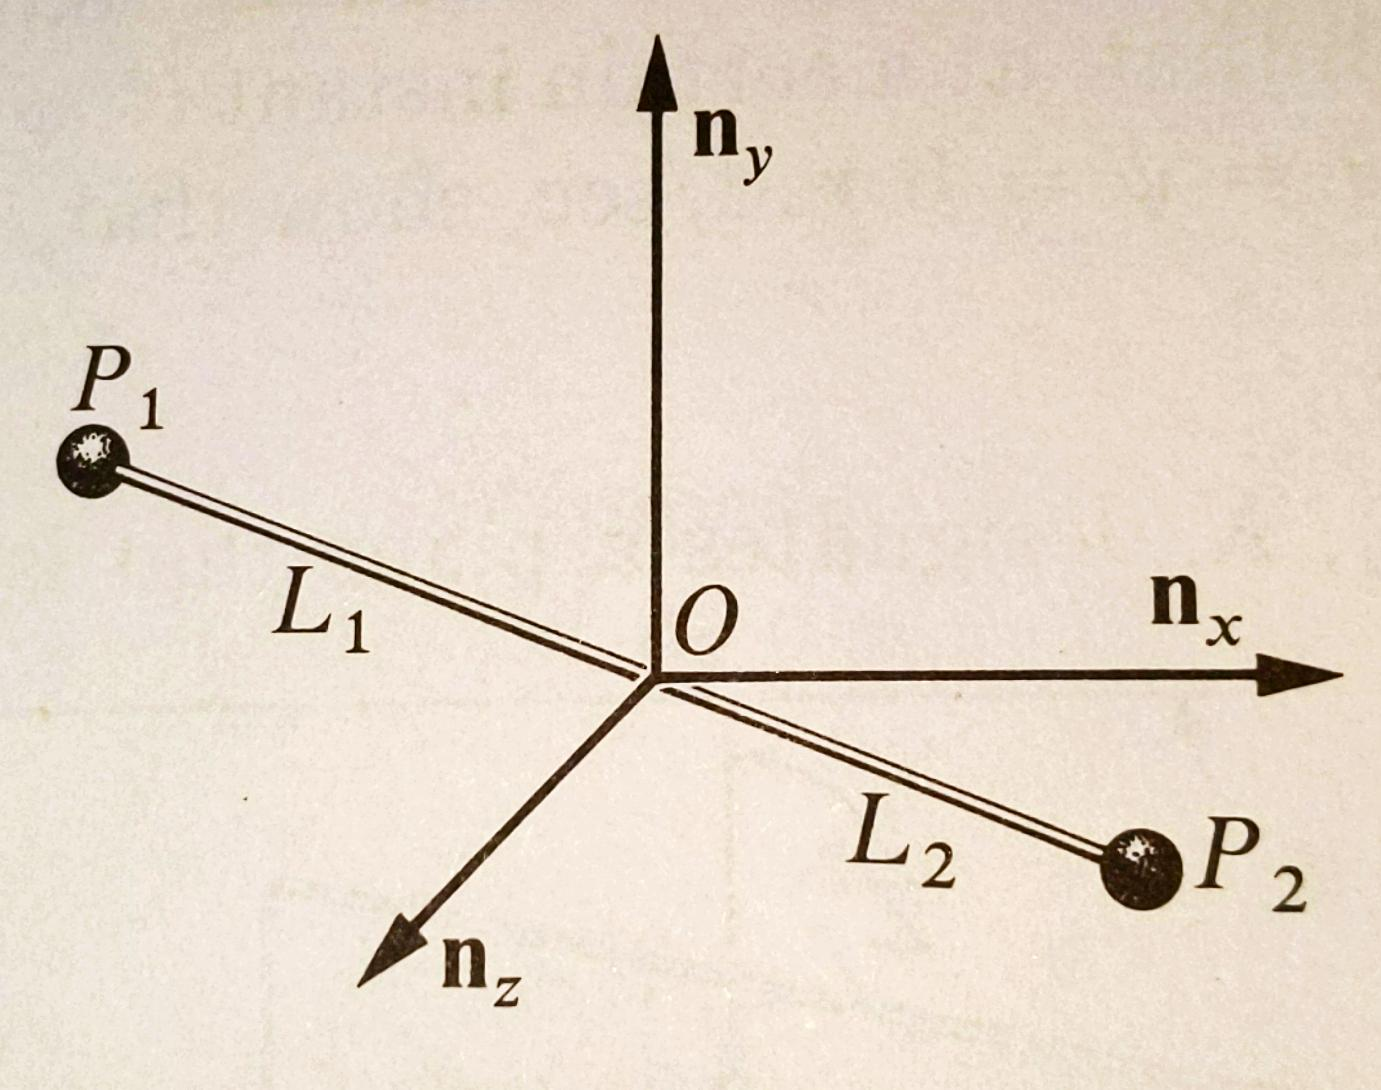
\includegraphics[scale = 0.15]{figs/ProbSet_1/1_e.jpg}
    \caption{}
    \label{1_e}
\end{figure}

Letting $\pmb p_1$ and $\pmb p_2$ be the position vectors of $P_1$ and $P_2$ relative to point $O$, and taking,

$$\pmb p_i = x_i \pmb n_x + y_i \pmb n_y + z_i \pmb n_z \qquad i = 1, 2$$

construct five constraint eqautions governing the six quantities $x_i, y_i, z_i$ for $i=1, 2$.

\itbf{Sol.}:
\begin{itemize}
    \item The system rotates in only x-y plane.
        \begin{align*}
            z_1 &= z_2 = 0 &\hdots 1, 2
        \end{align*}
    \item The distance from origin remain the same.
    \begin{align*}
        x_1^2 + y_1^2 &= L_1^2  &\hdots 3\\
        x_2^2 + y_2^2 &= L_2^2  &\hdots 4
    \end{align*}

    \item $P_1$ and $P_2$ lie on the same straight line, i.e., the slopes are equal. Let,
    \begin{align*}
        \sin \theta &= \frac{-y_1}{L_1} = \frac{y_2}{L_2} = \sqrt{\frac{y_1 y_2}{-L_1 L_2}}\\
        \cos \theta &=  \frac{x_1}{L_1} = \frac{x_2}{L_2} = \sqrt{\frac{x_1 x_2}{-L_1 L_2}}\\
        \text{Substituting into: }\quad
        \sin^2 \theta + \cos^2 \theta &= 1\\
        \implies x_1 x_2 + y_1 y_2 &= -L_1 L_2 &\hdots 5
    \end{align*}
\end{itemize}
